
V tejto časti popíšeme niekoľko algoritmov, ktoré sú pomerne úspešné
na praktických inštanciách problému, ale väčšinou je ich teoretická
analýza pomerne ťažká. Popíšeme niekoľko heuristík, ktoré v pomerne krátkom čase
dávajú riešenie, ktoré je väčšinou blížko optimálneho. Aby sme vedeli odhadnúť
kvalitu týchto heuristík, najprv ale ukážeme niekoľko algoritmov na hľadanie dolného odhadu
veľkosti riešenia. Následne ešte vylepšíme algoritmus používajúci
celočíselné lineárne programovanie od \cite{duchenne}, aby
sme dokázali optimálne riešiť inštancie, ktoré majú najviac 400 vrcholov.

\section{Dolné odhady veľkosti riešenia}

\subsection{Odhad pomocou dvoch disjuktných kostier}

Pomerne priamočiarym dolným odhadom veľkosti riešenia je veľkosť
dvoch nakratších disjuktných kostier. My to jemne vylepšíme budeme používať
tzv. 1-kostry.

\begin{definicia}
1-kostra v grafe $G=(V, E)$ je zjednotenie kostry na vrcholoch $V \setminus \{1\}$
a dvoch hrán susedných s vrcholom $1$. 
\end{definicia}

\begin{lema}
Veľkosť dvoch najlacnejších disjuktných 1-kostier je najviac tak veľká ako dĺžka
riešenia problému dvoch obchodných cestujúcich.
\end{lema}

\begin{dokaz}
Každá hamiltonovská kružnica je 1-kostra. Riešenie problému dvoch obchodných cestujúcich
sú teda dve disjuktné 1-kostry.
\end{dokaz}

Dve najkratšie disjuktné 1-kostry môžeme hľadať v čase $O(m \lg m + n^2)$ pomocou algoritmu popísaného v
\cite{spanning2} -- nájdeme najkratšie disjuktné kostry na $V \setminus \{1\}$ a k vrcholu $1$ ešte
pridáme štyri najkratšie hrany.

Tento odhad sa dá vylepšiť pomocou techniky opísanej v \cite{heldtsp} a \cite{lower1}.
Jej princíp je nasledovný. Každému vrcholu prirádíme potenciál 
$p_i \in \mathbb{R}$.
A zavedenieme nové dĺžky hrán:
$$d(u, v) = c(u, v) + p_u + p_v$$

\begin{lema}
Majme potenciály $p_1, p_2, \dots, p_n$. Riešenie problému dvoch obchodných
cestujúcich pri dĺžkach $d(u,v)$ definovaných vyššie je rovnaké ako riešenie
problému dvoch obchodných cestujúcich pri dĺžkach $c(u,v)$.
\end{lema}

\begin{dokaz}
Majme hamiltonovskú kružnicu $v_1, v_2, \dots, v_n$ s dĺžkou $C = c(v_1, v_2) + c(v_2, v_3) +
\dots + c(v_n, v_1)$. Pokiaľ zavedieme dĺžky hrán $d(u,v)$ dostaneme cenu:
$$C^{'} = c(v_1, v_2) + p_{v_1} + p_{v_2} + c(v_2, v_3) + p_{v_2} + p_{v_3} + \dots +
c(v_n, v_1) + p_{v_n} + p_{v_1}$$
$$C^{'} = C + 2 \sum_{v \in V} p_v$$

To znamená, že ku dĺžke každej hamiltonovskej kružnice prirátame rovnaké číslo
a teda najlepšie riešenie pri upravených dĺžkach je rovnaké ako najlepšie
riešenie pri pôvodných dĺžkach.
\end{dokaz}

Podstatné je, že zmenou potenciálov vieme zmeniť najlacnejšie disjuktné 1-kostry. 
Našim cieľom bude nájsť také potenciály, aby rozdiel medzi dĺžkou najlacnejších
disjuktných 1-kostier a dĺžkou riešenia problému dvoch obchodných cestujúcich
bol čo najmenší. Nech $C$ je dĺžka riešenia problému dvoch obchodných cestujúcich
pri nulových potenciáloch. Nech $D$ je dĺžka dvoch najlacnejších disjuktných 1-kostier
pri potenciáloch $p_1, \dots, p_n$. Potom spomínaný rozdiel vieme vyjadriť ako:
$$C + 2 \sum_{v \in V} p_v - D$$

V našom prípade je $C$ nám neznáma konštanta a teda stačí minimalizovať výraz:
$$2 \sum_{v \in V} p_v - D$$

Vhodné potenciály vieme nájsť napríklad pomocou subgradientovej optimalizácie.
Dá sa totiž ukázať, že ak $d_v$ je súčet stupňov vrchola $v$ v obidvoch kostrách, tak
vektor so zložkami $g_v = 4 - d_v$ je subgradient pre vyššie spomínaný optimalizačný
problém.

Algoritmus optimalizácie sa dá popísať nasledovne. Na začiatku položíme všetky potenciály
ako $p^{(0)}_v = 0$. V $i$-tej iterácii si najprv zvolíme veľkosť kroku $t^{(i)}$. Následne
spočítame subgradienty $g^{(i)}_v = 4 - d^{(i-1)}_v$ a následne vyrátame nové potenciály ako:
$p^{(i)}_v = p^{(i-1)}_v + t^{(i)} g^{(i)}_v$. V našej implementácii sme $t^{(i)}$ volili ako
konštantu a iterácie opakovali dovtedy, kým sa výsledok zlepšoval.

\subsection{Dolný odhad pomocou štyroch najbližších susedov}

Ešte ukážeme jeden dolný odhad, ktorý je o trochu rýchlejší ako odhad pomocou kostier a navyše má
niektoré príjemné vlastnosti, ktoré sa ukážu neskôr.

\begin{definicia}
Daný je ohodnotený graf $G = (V, E)$. Graf $k$ najbližších susedov $G_s = (V, E)$ je orientovaný
graf taký, že z každého vrchola $v \in V$ vychádza $k$ najkratších hrán, ktoré s vrcholom $v$
susedia v $G$. 
\end{definicia}

\begin{lema}
Nech $s$ je celková dĺžka hrán v grafe $4$ najbližších susedov, nech $f$ je dĺžka najlacnejšieho
$4$-faktora a $t$ je dĺžka riešenia problému dvoch obchodných cestujúcich. Potom:
$$ \frac{1}{2} s \leq f \leq t$$
\end{lema}

\begin{dokaz}
Druhá nerovnosť vyplýva z toho, že dve hamiltonovské kružnice tvoria dokopy 4-faktor.
Prvá nerovnosť vyplýva z toho, že keď z každej hrany 4-faktoru spravíme dve orientované hrany, tak
dostaneme graf v ktorom z každého vrchola vychádzajú práve 4 hrany.
\end{dokaz}

My budeme hľadať graf $4$ najbližších susedov. Vieme ho nájsť pomerne priamočiaro v čase lineárnom
od počtu hrán. Opäť môžeme použiť aj transformáciu pomocou potenciálou. Cieľom je tento krát
dostať hodnotu $s/2$ čo najbližšie k hodnote $f$ (keďže najlacnejší 4-faktor sa pri zmene
potenciálov nezmení). Celý postup subgradientovej optimalizácie je rovnaký ako pri disjuktných
1-kostrách.

\begin{poznamka}
Vedeli by sme aj priamo hľadať najlacnejší $4$-faktor prevedením na hľadanie najlacnejšieho
$1$-faktora v správne pozmenenom grafe. Výhoda nášho prístupu sa ukáže neskôr, keď budeme
vyhľadávať hrany, ktoré zaručene nepoužijeme v optimálnom riešení.
\end{poznamka}

\section{Heuristiky na hľadanie horného odhadu veľkosti riešenia}

Na hľadanie horného odhadu veľkosti riešenia použijeme upravenú Lin-Kernighanovu heuristiku pre
problém obchodného cestujúceho (\cite{link}). Táto heuristika postupne vylepšuje nájdené
riešenie pomocou lokálnych zmien. V každom kroku vyberie množinu $k$ hrán $X$, ktoré z aktuálneho
riešenia odstráni a množinu $k$ hrán $Y$, ktorú do riešenia pridá. Tejto operácii sa zvykne
hovoriť aj $k$-opt krok, v našej implementácii budeme používať $k$ maximálne 5.
Lin-Kernighanova heuristika kladie na tieto množiny ešte niekoľko obmedzení:

\begin{itemize}
\item Hrany z $X \cup Y$ musia tvoriť cyklus. Kroku, ktorých spĺňa túto podmienku
hovoríme aj sekvenčný $k$-opt krok. Na tomto cykle sa striedavo budú vyskytovať hrany z množín
$X$ a $Y$.
\item Hrany z $Y$ musia byť podmnožinou tzv. množiny kandidátov. Množina kandidátov je množina hrán,
o ktorej predpokladáme, že väčšina z hrán riešenia bude práve z nej. Obvykle je množina kandidátov
tvorená tak, že pre každý vrchol zoberieme $m$ najkratších hrán, ktoré s ním susedia. V našej
implementácii sme položili $m = 8$.
\end{itemize}

\begin{figure}[h]
\centering
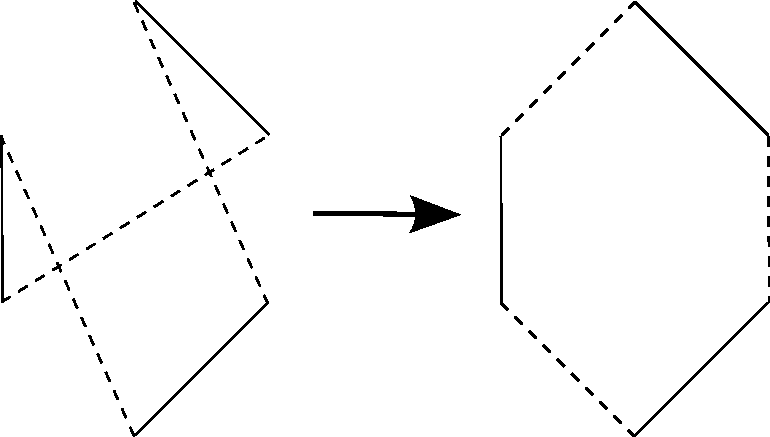
\includegraphics[scale=0.6]{img/opt3.pdf}
\caption{3-opt krok, čiarkovane sú vyznačené hrany, ktoré odstraníme, resp. pridáme}
\end{figure}


Sekvenčné $k$-opt kroky vieme hľadať priamočiaro pomocou rekurzie -- v každom kroku si vyberieme,
ktorú hranu pridáme do množiny $X$ alebo $Y$ (postupujeme striedavo), začíname najprv množinou $X$.
Po pridaní hrany do množiny $X$ skúsime uzavrieť cyklus (ignorujeme, či hrana, ktorá uzavrie
cyklus je z množiny kandidátov). A skontrolujeme, či po takomto ťahu dostaneme stále hamiltonovskú
kružnicu a či jej dĺžka bude kratšia. V momente, keď nájdeme vhodný ťah aplikujeme ho -- t.j.
nehľadáme najlepší $k$-opt ťah.

Zároveň si pri rekurzii počítame doterajší zisk, t.j. rozdiel medzi dĺžkou odobraných a pridaných hrán.
Pokiaľ chceme, aby náš $k$-opt krok bol dobrý, tak jeho zisk musí byť kladný. My použijeme ešte
agresívnejšie orezanie -- požadujeme, aby po každom kroku rekurzie sme malý kladný zisk. Toto vôbec
neobmedzí prehľadané kroky, lebo ak máme celkovo kladný zisk, tak vieme cyklus prejsť v takom
poradí, aby bol zisk po každom kroku kladný.

\medskip

V našom prípade máme hamiltonovské kružnice dve. Priamočiara implementácia by mohla pre každý
$k$-opt ťah kontrolovať, či neporuší podmienku disjuktnosti ciest a povoliť len tie, ktoré ju
neporušujú.

Naše kroky budú mierne komplikovanejšie. Algoritmus na ich nájdenie by sa dal popísať nasledovne:
\begin{enumerate}
\item Nájdi $k$-opt krok v jeden z kružníc, ktorý túto kružnicu zlepší. Nech tento krok vymaže hrany
z množiny $X$ a pridá hrany z množiny $Y$.
\item Ak sa žiadna hrana z množiny $Y$ nenachádza v druhej kružnici, vykonaj tento krok.
\item Ak má prienik druhej kružnice a $Y$ veľkosť 1, tak nájdi v druhej kružnici najlacnejší $2$-opt
alebo $3$-opt krok, ktorý obsahuje túto hranu. Ak sa po vykonaní týchto krokov zlepší súčet dĺžok
kružníc, vykonaj tieto kroky.
\item V prípade, že má tento prienik veľkosť viac ako $1$, označme hrany v prieniku ako $e_1, \dots,
e_k$. Tieto hrany nám druhú kružnicu rozdelia na niekoľko ciest. Vyskúšame všetky možnosti ako tieto
cesty pospájať bez toho, aby sme použili hrany $e_1, \dots, e_k$ a vyberieme najlacnejšiu. Ak sa po
vykonaní týchto krokov zlepší súčet dĺžkov kružníc vykonaj tieto krokov.
\item Ináč nájdi iný $k$-opt krok v prvej kružnici.
\end{enumerate}

Tieto kroky opakujeme kým sa riešenie nedá zlepšiť. Pokiaľ sa zasekneme v lokálnom optime, tak sa pokúsime 
dostať tak, že spravíme niekoľko krokov, ktoré jednu cestu zlepšia a súcet nezhoršia o viac ako
$1\%$. A následne sa opäť snazíme znižovať celkovú dĺžku. Algoritmus skončí vtedy, keď sa už ani
po takýchto krokoch nepodarí riešenie zlepšiť.

\section{Riešenia pomocou celočíselného lineárneho programovania}

Naše riešenie vychádza z riešenia od \cite{duchenne}, ktoré sme stručne opísali v druhej kapitole.
Pripomeňme, že hlavnou myšlienkou tohoto riešenia je hľadať 4-súvislý 4-faktor, ktorý sa následne
pokúšeme rozdeliť na dve hamiltonovské kružnice. Pokiaľ sa toto rozdelenie nepodarí, daný 4-faktor
zakážeme a hľadáme ďalší.

My toto riešenie vylepšíme pomocou niekoľkých vecí.

\subsection{Rozdeľovanie 4-súvislého 4-faktora pomocou SAT solvera}

Ako sme už spomínali zistiť, či sa dá rozdeliť 4-súvislý 4-faktor na dve hamiltonovské kružnice
je NP-úplný problém. Pôvodné riešenie tento problém rieši pomocou celočíselného lineárneho programu.
Keďže ale tento problém je rozhodovací a nie optimalizačný, nám sa zdá rozumnejšie tento 
problém riešiť pomocou SAT solvera. Technika riešenia bude takmer podobná ostatným.
Na začiatku budeme požadovať iba rozklad na dva 2-faktory (t.j. rozložíme hrany do dvoch množín $A,
B$ tak, aby každý vrchol mal dve susedné hrany z $A$ a dve susedné hrany z $B$). Pokiaľ sa vyskytne
nejaký cyklus $C$, ktorý neprechádza celým grafom, tak tento cyklus zakážeme (t.j. budeme požadovať
výskyť aspoň jednej hrany medzi množinami $C$ a $V \setminus C$). 

\subsection{Zrýchlenie rozdeľovania pomocou hľadania vhodných podgrafov}

Už \cite{duchenne} ukázal jeden spôsob ako zrýchliť rozhodovanie, či sa dá 4-súvislý 4-faktor
rozdeliť na dve hamiltonovské kružnice.

\begin{definicia}
Artikulačný pár v 4-súvislom 4-regulárnom grafe $G = (V, E)$ 
je dvojica vrcholov $v_1, v_2$ také, že keď z grafu odstránime
tieto vrcholy a ich susediace hrany, tak sa graf rozpadne na dva grafy
$G_1, G_2$.
\end{definicia}

Artikulačné páry vieme triviálne hľadať v čase $O(n^3)$.

Pokiaľ nájdeme v grafe $G$ artikulačný pár $v_1, v_2$ môžeme ho rozdeliť pomocou nasledovnej
dekompozície:
Nech sa po odstránení vrcholov $v_1, v_2$ graf rozpadne na dva grafy $G_1, G_2$.
Graf $G_1^{'}$ vytvoríme z $G_1$ tak, že mu pridáme vrcholy $v_1, v_2$ a všetky hrany, ktoré spajáli
vrcholy $v_1, v_2$ s grafom $G_1$ v grafe $G$. Následne ešte spojíme vrcholy $v_1, v_2$ medzi sebou
pomocou dvoch hrán. Obdobne vyrobíme z grafu $G_2$ graf $G_2^{'}$.

\begin{figure}
\centering
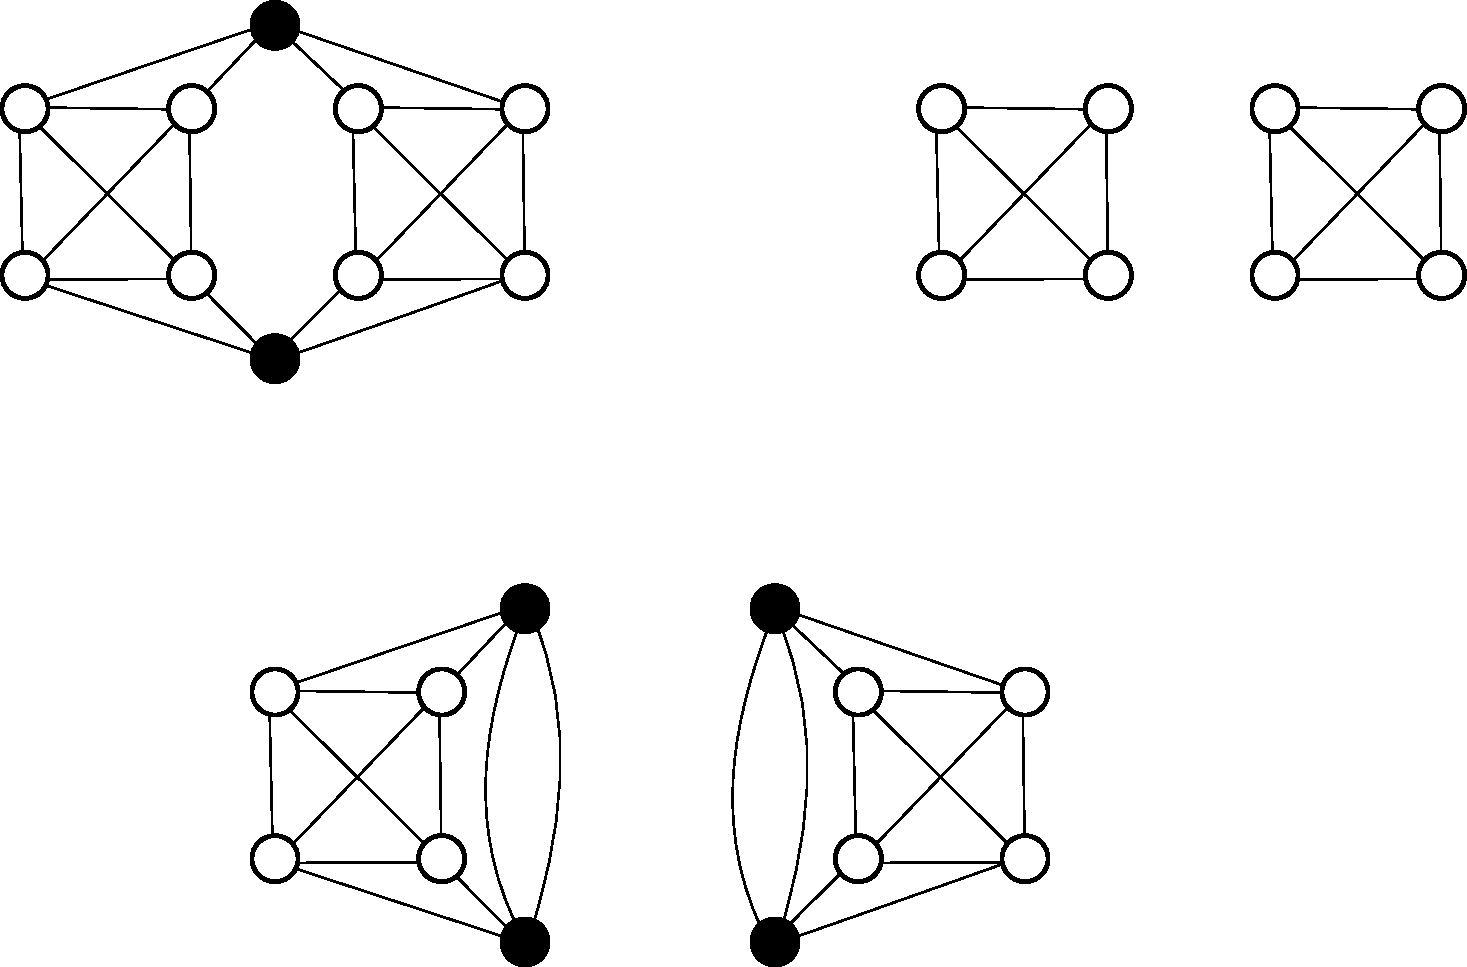
\includegraphics[width=15cm]{img/decomp.pdf}
\caption{Dekompozícia grafu. Hore vľavo: vstupný graf $G$ s vyznačeným artikulačným párom. Hore
vpravo: Graf po odstranení artikulačného páru. Dole: Vzniknuté grafy, po pridaní artikulačným párov
a hrán medzi nimi.}
\end{figure}

Grafy $G_1^{'}, G_2^{'}$ budú 4-súvislé a 4-regulárne. Navyše o nich platí nasledovné.

\begin{veta}
Nech $G$ je 4-súvislý 4-regulárny graf, ktorý obsahuje artikulačný pár $v_1, v_2$.
Nech $G_1^{'}, G_1^{'}$ sú grafy, ktoré vznikli dekompozíciou popísanou vyššie.
Graf $G$ sa dá rozložiť na dve hamiltonovské kružnice práve vtedy a len vtedy, keď
sa grafy $G_1^{'}$ a $G_2^{'}$ dajú rozložiť na dve hamiltonovské kružnice.
\end{veta}

\begin{dokaz}
Pozri \cite{duchenne}.
\end{dokaz}

Túto techniku môžeme aplikovať rekurzívne. Navyše pokiaľ sme spravili iba jednu dekompozíciu, tak
môžeme zakázať menšiu časť grafu ako celý. T.j. ak sa nepodarí daný graf $G$ rozložiť na dve
hamiltonovské kružnice, preto, lebo graf $G_1^{'}$ sa nepodarilo rozložiť, tak môžeme miesto podmienky:
$$\sum_{e \in G} x_e \leq 2n - 1$$

Použiť podmienku:
$$\sum_{e \in G_1^{'}} x_e \leq |E_1^{'}| - 1$$

Táto podmienka hovorí, že daný graf potrebujeme zmeniť.
Táto technika ale nefunguje rekurzívne, ale iba pri prvej dekompozícii. Protipríklade môžeme vidieť
na obrázku \ref{TODO}. Po troch krokoch dekompozície by sme zistili, že problematický je graf $G_1$.
Avšak riešenie sa dá dosiahnúť ak tak, že graf $G_1$ nezmeníme, ale prepojíme medzi sebou napríklad
grafy $G_2$ a $G_3$.

TODO obrázok



\medskip

V našom algoritme používame ešte jednu operáciu, ktorá vstup pre SAT solver ešte zjednoduší.
Myšlienka vyzerá nasledovne: Ak nájdeme nejakú štvorcu bodov, ktoré sú všetky navzájom spojené
(kliku veľkosti 4), tak
ich môžeme zlučiť do jedného bodu.

\begin{veta}
Nech $G$ je 4-súvislý 4-regulárny graf a nech $v_1, v_2, v_3, v_4$ sú jeho vrcholy také, že medzi
každými dvoma vedie hrana. Nech graf $G^{'}$ vznikne z grafu $G$ tak, že vrcholy $v_1, v_2, v_3,
v_4$ zlúčime do jedného. Potom graf $G$ je rozložiteľný na dve hamiltonovské kružnice práve vtedy a
len vtedy, keď je graf $G^{'}$ rozložiteľný na dve hamiltonovské kružnice.
\end{veta}

\begin{dokaz}
Zoberme hrany, ktoré vedú medzi množinami $V_x = \{v_1, v_2, v_3, v_4\}$ a $V \setminus V_x$.
Takéto hrany sú práve 4. Ak by ich bolo menej, tak $G$ nie je 4-súvislý, ak by ich bolo viac, tak
$G$ nemôže byť 4-regulárny.

Ak sa graf $G$ dá rozložiť na dve hamiltonovské kružnice, tak triviálne vidno, že aj graf $G^{'}$ sa
dá rozložiť (kružnice budú presne rovnaké akuráť vynecháme hrany medzi vrcholmi $v_1, \dots, v_4$).

\begin{figure}[h]
\centering
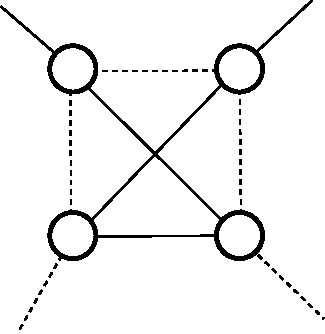
\includegraphics[scale=0.5]{img/k4.pdf}
\caption{Prechod kružníc cez kliku veľkosti 4}
\label{fig:k4}
\end{figure}

Ak sa graf $G^{'}$ dá rozložiť na dve hamiltonovské kružnice, tak pomocou vhodného prepojenia (viď.
\ref{fig:k4}) medzi
vrcholmi $v_1, \dots, v_4$ vieme graf $G$ rozložiť na dve hamiltonovské kružnice (ostatné hrany
rozložíme medzi kružnice rovnako ako v grafe $G^{'}$).
\end{dokaz}

Poznamenajme, že takéto štvorice vrcholov vieme hľadať v čase $O(n)$ -- vyberieme si jeden vrchol
$v_1$ a v konštantom čase prejdeme všetky jeho kombinácie susedov.

\subsection{Odstráňovanie nepoužiteľných hran}

Predstavme si graf, ktorého vrcholy zodpovedajú bodom v rovine. Pomerne intuitívne vieme označiť
veľa hrán, o ktorých si sme istý, že v optimálnom riešení určite nebudú -- sú to hlavne tie hrany,
ktoré vedú cez celú rovinu. My by sme v tejto časti chceli ukázať ako tieto hrany
hľadať algoritmicky. Pokiaľ by sme ich vedeli hľadať, môžeme obmedziť počet premenných, ktoré
sú v lineárnom programe a tak urýchliť jeho riešenie.

\begin{lema}
Nech $l(G, e)$ je dolný odhad veľkosti riešenia, ktoré obsahuje hranu $e$.
Nech $u(G)$ je nejaký horný odhad riešenia. Ak $l(G, e) > u(G)$, tak sa hrana $e$ určite nepoužije v
optimálnom riešení.
\end{lema}

\begin{dokaz}
Triviálny.
\end{dokaz}

Ako získať horný odhad veľkosti riešenia sme už popísali. Ešte potrebujeme popísať ako získať dolný
odhad, ktorý obsahuje hranu $e$.

\medskip
Pokiaľ používame dolný odhad pomocou štyroch najbližších susedov, tak sa dolný odhad, ktorý obsahuje
hranu $e$ dá získať pomerne jednoducho. Nech $e$ vedie medzi vrcholmi $x, y$. Potom do veľkosti
dolného odhadu miesto $4$ najbližších susedov započítame iba $3$ najbližších susedov (okrem hrany
$e$) a navyše hranu $e$ započítame $2-krát$. Pokiaľ máme už dopredu spočítaný dolný odhad bez nutnej
hrany, tak pre danú hranu $e$ vieme tento odhad prerátať v konštantnom čase. 
To znamená, že v čase $O(n^2)$ vieme nájsť nepoužiteľné hrany. 

\medskip
Pokiaľ používame dolný odhad pomocou dvoch disjuktných kostier, tak je situácia trochu zložitejšia.
Pokiaľ máme spočítané najlacnejšie dve disjuktné kostry a chceme, aby sa nutne použila hrana $e$,
tak potrebujeme z týchto kostier jednu hranu vyhodiť. Nestačí sa ale len pozrieť na cykly v ktorých
leží hrana $e$, lebo môžeme si hrany medzi kostrami presúvať. To znamená, že vložime hranu $e$, inú
hranu $e_1$ presunieme z kostry $M_1$ do kostry $M_2$ ($e$ a $e_1$ ležali po pridaní do $M_1$ na
jednom cykle), ďalšiu hranu $e_2$ presunieme z $M_2$ do $M_1$, atď., až nakoniec odstraníme hranu
$e_k$. Teda hľadáme cestu medzi hranami kostier a chceme vyhodiť najlacnejšiu hranu, ku ktorej sa
vieme dostať. Tento problém efektívne rieši značkovacia procedúra z \cite{spanning2}, akurát si
potrebujeme pamätať akú najlacnejšiu hranu vieme dosiahnúť. Táto značkovacia procedúra trvá pre
jednu hranu čas $O(n)$. Následne keď zistíme, ktorú hranu musíme z kostier vyhodiť, tak
veľkosti dolného odhadu vieme prerátať triválne. Celkovo na to, aby sme o každej hrane zistili či
je zbytočná potrebujeme čas $O(n^3)$. 

\begin{poznamka}
Dobre spravený algoritmus by toto vedel riešiť aj v čase $O(n^2)$. Keďže ale vo všetkých
naších vstupoch platí $n \leq 500$, tak je $O(n^3)$ riešenie postačujúce a nepotrebujeme sa zaoberať
komplikovanejším riešením.
\end{poznamka}

\section{Experimenty}

Vyššie popísané algoritmy sme implementovali s cieľom empiricky overiť ich účinnosť na
niektorých druhoch dát. Testovacie dáta budú tvoriť náhodné grafy v euklidovskej rovine (kde
súradnice bodov sú vyberané rovnomerne náhodne) a niektoré inštancie z TSPLIB (\cite{tsplib}).

Hľadanie dolných a horných odhadov sme implementovali v C++. Na riešenie celočíselných
lineárnych programov sme použili Numberjack, ktorý používa SCIP a ako SAT solver sme použili knižnicu STP, ktorá
používa MINISAT. Réžiu okolo celočíselných lineárnych programov a SAT solvera sme
implementovali v jazyku Python. Algoritmy sme testovali na počítači s procesorom
Intel i7 Q720. 

Testovali sme tri rôzne implementácie. Jedna nepoužívala žiadne vyhadzovanie nepotrebných
hrán, druhá používala vyhadzovanie nepotrebných hrán cez štyroch najbližších susedov a tretia
používala vyhadzovanie nepotrebných hrán pomocou dvoch disjuktných kostier.

V prípade náhodných grafov v euklidovskej rovine sme generovali grafy veľkosti $100$, $150$, $200$,
$250$, $300$. Pre každú veľkosť sme vygenerovali 10 grafov.
Následne sme každú našu implementáciu pustili a sledovali niekoľko údajov:
\begin{itemize}
\item Či úspešne skončí do jednej hodiny. Ak neskončí, tak rátame riešenie za neúspešné.
\item Ako rýchlo skončí.
\item Koľko krát sa vykoná rozklad 4-súvislého 4-faktora na dve hamiltonovské kružnice.
\item Koľko hrán bolo označených ako nepoužiteľné.
\end{itemize}

\subsection{Výsledky pre náhodné grafy v euklidovskej rovine}

V tabuľke \ref{table1} sú zhrnuté priemerné výsledky pre každú veľkosť grafu.
Označenia: 
\begin{myitemize}
\item $n$ -- veľkosť grafu
\item $f_a$ -- priermerný počet rozkladov na dve hamiltonovské kružnice pre všetky
inštancie (v prípade, že sme do hodiny nedostali výsledok, tak rátame počet rozkladov, ktoré program
stihol vykonať za hodinu)
\item $f_u$ -- priemerný počet rozkladov pre inštancie, kde sme úspešne skončili
\item $f_1$ -- počet inštancií, kde prvý rozklad bol úspešný 
\item $s_n$ -- uspešnosť algoritmu, keď sme žiadne nepotrebné hrany nehľadali
\item $t_n$ -- priemerný čas behu algoritmu, keď sme žiadne nepotrebné hrany nehľadali (pokiaľ sme
neskončili v priebehu hodiny, do priemeru zarátame hodinu) v sekundách
\item $u_n$ - to isté, čo $t_u$ ale rátame priemer iba na inštanciách, kde sme úspešne skončili
\item $s_4, t_4, u_4$ -- úspešnosť a časy behu v prípade, že nepoužiteľné hrany, hľadáme pomocou
štyroch najbližších susedov
\item $d_4$ -- priemerný podiel nájdených nepoužíteľných hrán
\item $s_k, t_k, u_k$ -- úspešnosť a časy behu v prípade, že nepoužiteľné hrany, hľadáme pomocou
dvoch disjuktných kostier
\item $d_k$ -- priemerný podiel nájdených nepoužíteľných hrán
\end{myitemize}



\begin{table}[h]
\centering
\begin{tabular}{|r|r|r|r|r|r|r|r|r|r|r|r|r|r|r|}
\hline
$n$&$f_a$&$f_u$&$f_1$&$s_n$&$t_n$&$u_n$&$s_4$&$t_4$&$u_4$&$d_4$&$s_k$&$t_k$&$u_k$&$d_k$ \\\hline
100& 57  & 29  & 5   & 0.9 & 736 & 378 & 0.9 & 687 & 322 & 0.64& 0.9 & 585 & 249 & 0.70 \\\hline
150& 83  & 28  & 4   & 0.7 & 1380& 428 & 0.7 & 1327& 353 & 0.61& 0.7 & 1314& 334 & 0.58 \\\hline
200& 68  & 8   & 3   & 0.5 & 2000& 400 & 0.5 & 1903& 206 & 0.56& 0.5 & 1913& 226 & 0.60 \\\hline
250& 46  & 22  & 2   & 0.3 & 2769& 819 & 0.4 & 2662& 1255& 0.50& 0.4 & 2615& 1136& 0.57 \\\hline
300& 34  & 6   & 0   & 0.2 & 3087& 1035& 0.2 & 3029& 745 & 0.52& 0.2 & 3021& 705 & 0.52 \\\hline
\end{tabular}
\caption{Výsledky pre náhodné grafy.}
\label{table1}
\end{table}

Z tabuľky sa dá usúdiť niekoľko záverov.

Vidíme, že odhad pomocou dvoch kostier odstráni o niečo viac hrán ako odhad pomocou štyroch najbližších susedov
Z hľadiska celkového času sú tieto algoritmy
porovnateľné. Ďalej vidíme, že odstráňovanie týchto hrán sa opláca (pri veľkosťi 250 je menší
čas pri neorezávaní spôsobený tým, že zarátavame iba 3 inštancie namiesto 4).

V porovnaní s \cite{duchenne} máme o niečo vyššiu úspešnosť, oni pri inštanciách
veľkosti $190$ dosahujú úspešnosť $0.2$ a pre väčšie inštancie vyzerá, že sú neúspešní.
My túto hranicu posúvame na $300$.

\subsection{Výsledky pre niektoré inštancie z TSPLIB}

Výsledky pre inštancie z TSPLIB zhŕňa nasledujúca tabuľka. 
Označenia (uvádzame iba iné ako v predchádzajúcej tabuľke a miesto priermerných časov uvádzame čas
behu jednej inštancie):
\begin{myitemize}
\item Inst -- názov inštancie, číslo v názve vyjadruje počet vrcholov
\item $t_d$ -- čas riešenia uvádzaný v \cite{duchenne}, ak bol uvádzaný
\end{myitemize}

\begin{table}[h]
\centering
\begin{tabular}{|r|r|r|r|r|r|r|r|}
\hline
Inst    &$f_a$&$t_n$&$t_4$&$d_4$&$t_k$&$d_k$&$t_d$ \\\hline
kroA100 & 26  & 200 & 178& 0.66 & 187 & 0.73& -- \\\hline
kroB100 & 3   & 25  & 23 & 0.70 & 24  & 0.61& 209 \\\hline 
kroC100 & 5   & 45  & 41 & 0.65 & 43  & 0.67& 137 \\\hline
kroD100 & 1   & 14  & 16 & 0.70 & 18  & 0.90& 10 \\\hline
kroE100 & 1   & 8   & 10 & 0.73 & 16  & 0.68& 23 \\\hline
bier127 & 24  & 220 & 225& 0.08 & 219 & 0.63& -- \\\hline 
kroA150 & 1   & 18  & 26 & 0.55 & 20  & 0.85& 749 \\\hline
kroA200 & 1   & 65  & 67 & 0.50 & 50  & 0.73& 311 \\\hline
a280    & 1   & 201 & 203& 0.70 & 317 & 0.09& 3085 \\\hline
lin318  & 1   & 573 & 276& 0.34 & 276 & 0.29& -- \\\hline
rd400   & 1   & 813 & 857& 0.48 & 741 & 0.50& -- \\\hline
pcb442  & 1   & --  &1503& 0.20 & 1775& 0.23& -- \\\hline
\end{tabular}
\end{table}

Výsledky ukazujú, že náš algoritmus je rádovo rýchlejši ako algoritmus od \cite{duchenne}.
Naša najväčšia zriešená inštancia má veľkosť $442$, v ich prípade je to $280$.
Navyše sa ukazuje, že vymazávanie nepotrebných hrán pomáha, ale nie je to hlavný faktor nášho
zrýchlenia. Autori prechádzajúceho algoritmu hovoria, že drvivú väčšinu času ich algoritmus strávi
zistovaním, či je príslušný 4-súvislý 4-faktor rozložiteľný na dve hamiltonovské kružnice.
Preto sme zobrali niektoré inštancie z TSPLIB, ktoré boli rozložiteľné na prvý krat
a pustili ich na našom algoritme bez vyhadzovania hrán. Tentokrát sme nemerali celkový čas, ale
aké percento času algoritmus strávil hľadaním rozkladu na kružnice ($p_r$). Toto sme porovnali s
predchádzajúcimi výsledkami $p_d$. Pre prehľadnosť uvádzame aj časy riešenia.

\begin{table}[h]
\centering
\begin{tabular}{|r|r|r|r|r|}
\hline
Inst   & $p_r$ & $p_d$ & $t_n$ & $t_d$ \\\hline
kroD100& 0.43  & 0.90  & 14    & 10 \\\hline
kroE100& 0.71  & 1.00  & 8     & 23 \\\hline
kroA150& 0.35  & 0.95  & 18    & 749 \\\hline
kroA200& 0.44  & 0.93  & 65    & 311 \\\hline
a280   & 0.93  & 0.73  & 201   & 3085 \\\hline
lin318 & 0.22  & --    & 573   & -- \\\hline 
\end{tabular}
\end{table}

V tabuľky vidno, že náš algoritmus trávi oveľa menej času pri zistovaní, či je daný 4-súvislý
4-faktor rozložiteľný na dve hamiltonovské kružnice. To mu umožňuje vyriešiť aj niektoré inštancie,
ktoré toto potrebujú zistovať aj viac krát (napr. bier127).

\bigskip

Z týchto meraní teda vyplýva, že hlavnou výhodou nášho algoritmu je lepší algoritmus na rozkladanie
grafu na dve kružnice. V niektorých prípadoch vieme navyše algoritmus zrýchliť aj tým, že nájdeme
nepoužiteľné hrany, ale toto zrýchlenie je oveľa slabšie. Náš algoritmus vie riešiť náhodné
inštancie do veľkosti 300 a aj niektoré väčšie inštancie, pokiaľ sa mu ich podarí rozložiť na prvý
pokus.

Zaujímavou teoretickou otázkou aký očakávaný počet takýchto rozkladov pre rôzne $n$.
Táto otázka je pomerne príbuzná otázke: koľko percent 4-súvislých 4-regulárny grafov s $n$ vrcholmi
sa dá rozložiť na dve hamiltonovské kružnice. Bohužial nepodarilo sa nám nájsť žiadny odhad
na počet 4-súvislých 4-regulárnych grafov a teda na túto otázku odpovedať nevieme.

\section{Heuristiky pre väčšie inštancie}

Na webovej stránke Kaggle.com sa konala súťaž Travelling santa problem, v ktorej bola
zadaná inštancia problému dvoch obchodných cestujúcich s drobnými obmenami, ktorá mala
150000 vrcholov, ktoré predstavovali body v rovine. Spomínané obmeny boli:
\begin{itemize}
\item Cieľom nebolo nájsť disjuktné kružnice, ale disjuktné cesty, ktoré prechádzali
všetkými vrcholmi.
\item Cieľom nebolo minimimalizovať súčet dĺžok ciest, ale minimalizovať dĺžku dlhšej
cesty.
\end{itemize}

Do tejto súťaže sme sa zapoli spolu s Petrom Perešínim. Skončili sme na prvom mieste,
kde naše riešenie malo dĺžku $6526972$, pričom nami vyratány dolný odhad
mal veľkosť: $6525773$. To znamená, že sme boli od opmima vzdialený najviac
$1199$, čo je asi $0.02\%$.

Okrem techník spomenutých vyššie sme v tejto súťaži využili niekoľko ďalších heuristík:

Neriešili sme problém zo zadania, t.j. minimalizovať dĺžku dlhšej cesty, ale našim
cieľom bolo minimalizovať súčet dĺžok ciest. Zistili sme, že nie je problém zabezpečiť,
aby cesty mali takmer podobnú dĺžku (stačí niekoľko prehodení hrán medzi cestami) a preto
nám táto zmena nerobí veľký problém.

Robili sme dolný odhad priamo pomocou najmenšieho 4-faktoru. Tento sme rátali
pomocou celočíselného lineárneho programu. Navyše sme ho nemohli rátať priamo
pre inštanciu veľkosti $150000$. Preto sme danú inštanciu nasekali na menšie
obdĺžnikové kúsky a hľadali najmenší 4-faktor v nich. Nepríjemnou technickou
záležisťou bolo urobiť tento dolný odhad pre 2 cesty miesto 2 cyklov.

Pri riešení sme využívali aj vyššie spomínané celočíselné lineárne programovanie
spolu so SAT solverom. Opäť sme nechceli nájsť optimálne riešenie pre celú inštanciu,
ale optimálne riešenie pre nejakú danú časť.

Ešte sme používali jednu heuristiku. Jej kroky sa dajú zhrnúť nasledovne:
\begin{enumerate}
\item Spoj obidve cesty do jedného grafu (dostaneme takmer 4-regulárny graf)
\item V tomto grafe nájde alternujúcu kružnicu, ktorá má zápornú cenu (t.j. cena vložených
hrán je menšie ako cena odstránených hrán) a následne pomocou nej zmenší veľkosť
daného grafu.
\item Pokús sa graf spätne rozložiť na dve cesty.
\end{enumerate}

V kroku 2 sme hľadali pomerne dlhé alternujúce kružnice. Na toto sme opäť
použili heuristiku. Tak isto sme použili aj heuristiku na rozkladanie grafu
na dve cesty. Viac o týchto heuristikách sa dá nájsť v \cite{kaggle}. 
